\documentclass{beamer}
\usepackage{../common_slides}
\usepackage{tikz-qtree}
\usepackage{stackengine}
\stackMath
\newlength\matfield
\newlength\tmplength
\def\matscale{1.}
\newcommand\dimbox[3]{%
  \setlength\matfield{\matscale\baselineskip}%
  \setbox0=\hbox{\vphantom{X}\smash{#3}}%
  \setlength{\tmplength}{#1\matfield-\ht0-\dp0}%
  \fboxrule=1pt\fboxsep=-\fboxrule\relax%
  \fbox{\makebox[#2\matfield]{\addstackgap[.5\tmplength]{\box0}}}%
}
\newcommand\raiserows[2]{%
   \setlength\matfield{\matscale\baselineskip}%
   \raisebox{#1\matfield}{#2}%
}
\newcommand\matbox[4]{
  \stackunder{\dimbox{#1}{#2}{$#4$}}{\scriptstyle #3}%
}

\title{Part-of-Speech Tagging \\ + \\ Neural Networks 3: Word Embeddings}
\date{}
\author{CS 287}
\begin{document}


\begin{frame}
  \titlepage
\end{frame}


\begin{frame}{Review: Neural Networks}
  One-layer multi-layer perceptron architecture,

  \[NN_{MLP1}(\boldx) =  g(\boldx\boldW^1 + \boldb^1)\boldW^2 + \boldb^2\]
  \begin{itemize}
  \item $\boldx\boldW + \boldb$; \textit{perceptron}
  \item $\boldx$ is the dense representation in $\reals^{1 \times \din}$
  \item $\boldW^1 \in \reals^{\din \times \dhid}, \boldb^1 \in \reals^{1 \times \dhid}$; first affine transformation
  \item $\boldW^2 \in \reals^{\dhid \times \dout}, \boldb^2 \in \reals^{1 \times \dout}$; second affine transformation
  \item $g:\reals^{\dhid \times \dhid}$ is an \textit{activation non-linearity} (often pointwise)
  \item $g(\boldx\boldW^1 + \boldb^1)$ is the \textit{hidden layer}
  \end{itemize}
\end{frame}

\begin{frame}{Review: Non-Linearities Tanh}
  Hyperbolic Tangeant:
  \begin{figure}
    \centering
    \[\tanh(t) = \frac{\exp(t) - \exp(-t)}{\exp(t) + \exp(-t)}  \]
    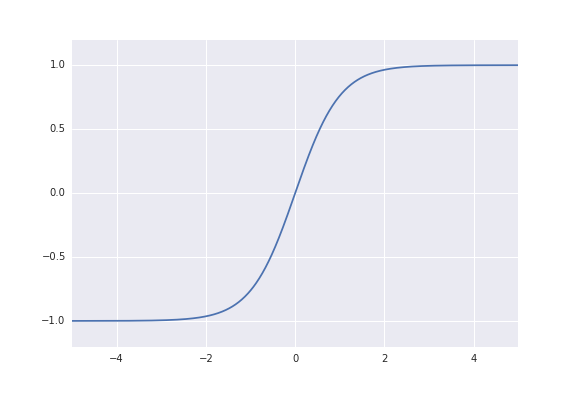
\includegraphics[width=5cm]{../notebooks/tanh}
    \includegraphics[width=5cm]{../notebooks/tanhgrad}
  \end{figure}
  \begin{itemize}
  \item Intuition: Similar to sigmoid, but range between 0 and -1.
  \end{itemize}
\end{frame}

\begin{frame}{Review: Backpropagation}
  \begin{center}

  \begin{tikzpicture}
    \node(x){$f_{i}(\ldots f_{1}(\boldx^0)) $};
    \node(t)[below right= of x, draw]{$f_{i+1}(*;\btheta_{i+1})$};

    \node(fx)[above right=of t]{$f_{i+1}(f_{i}(\ldots f_{1}(\boldx^0)))$};
    \node(gradin)[below left =of t]{$\displaystyle \frac{\partial L}{\partial f_i(\ldots f_1(\boldx^0))  } $};
    \node(gradout)[below right= of t]{$\displaystyle  \frac{\partial L}{\partial f_{i+1}(\ldots f_1(\boldx^0))  }  $};
    \node(gradweight)[below = of t, yshift=1cm]{$\displaystyle  \frac{\partial L}{\partial \btheta_{i+1}  }$};
    \path[draw, ->] (x) -> (t);
    \path[draw, ->] (t) -> (fx);
    \path[draw, ->] (t) -> (gradin);
    \path[draw, ->]  (gradout) -> (t);
  \end{tikzpicture}
  \end{center}
\end{frame}


\begin{frame}{Quiz}
  One common class of operations in neural network models is known as
  \textit{pooling}. Informally a pooling layer consists of aggregation
  unit, typically unparameterized, that reduces the input to a smaller
  size.
  \air

  Consider three pooling functions of the form $f: \reals^n \mapsto \reals$,
  \begin{enumerate}
  \item $ f(\boldx) = \max_{i} x_i $
  \item $ f(\boldx) = \min_{i} x_i $
  \item $ f(\boldx) = \sum_i x_i / n $
  \end{enumerate}
  \air

  What action do each of these functions have? What are their gradients?
  How would you implement backpropagation for these units?
\end{frame}

\begin{frame}{Quiz}
  \begin{itemize}
  \item \textbf{Max pooling}:  $f(\boldx) = \max_{i} x_i$

    \begin{itemize}
    \item Keeps only the most activated input
    \item Fprop is simple; however must store $\argmax$ (``switch'')
    \item Bprop gradient is zero except for switch, which gets gradoutput
    \end{itemize}
    \pause

  \item \textbf{Min pooling}: $ f(\boldx) = \min_{i} x_i $
    \begin{itemize}
    \item Keeps only the least activated input
    \item Fprop is simple; however must store $\argmin$ (``switch'')
    \item Bprop gradient is zero except for switch, which gets gradoutput
    \end{itemize}
    \pause

  \item \textbf{Avg pooling}: $ f(\boldx) = \sum_i x_i / n $
    \begin{itemize}
    \item Keeps the average activation input
    \item Fprop is simply mean.
    \item Gradoutput is averaged and passed to all inputs.
    \end{itemize}
  \end{itemize}
\end{frame}

\section{Embedding Motivation}

\begin{frame}
  \begin{center}
    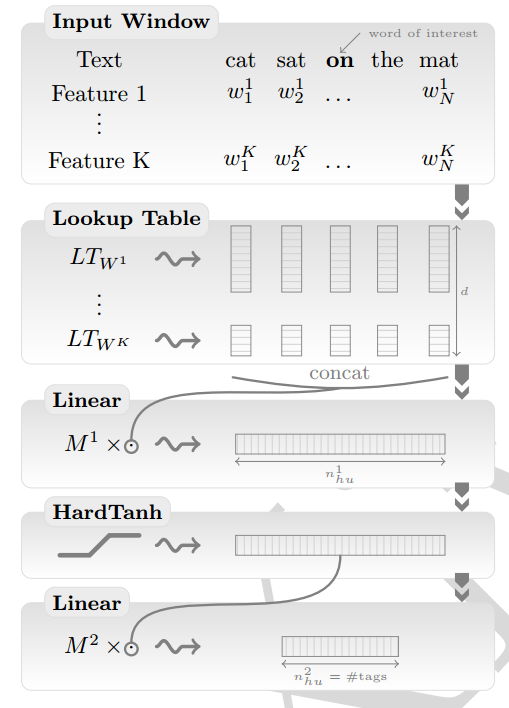
\includegraphics[width=5cm]{cwfull}
  \end{center}
  \begin{enumerate}
  \item Use dense representations instead of sparse
  \item Use windowed area instead of sequence models
  \item Use neural networks to model windowed interactions
  \end{enumerate}
\end{frame}


\begin{frame}{What about rare words?}
  \begin{center}
    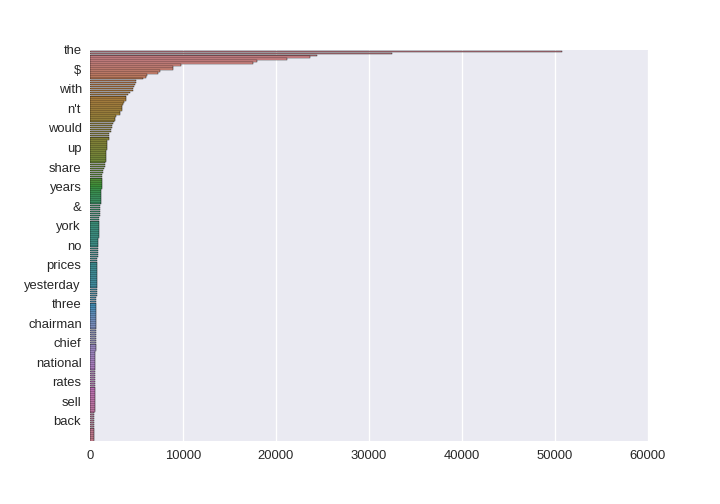
\includegraphics[width=0.8\textwidth]{../notebooks/zipf}
  \end{center}
\end{frame}

\begin{frame}{Word Embeddings}
  Embedding layer,
  \[ \boldx^0 \boldW^0 \]
  \begin{itemize}
  \item $\boldx^0 \in \reals^{1 \times d_0}$ one-hot word.
  \item $\boldW^0 \in \reals^{d_0 \times \din}$, $d_0 = |\mcV|$
  \end{itemize}
  \air
  Notes:
  \begin{itemize}
  \item $d_0 >> \din$, e.g. $d_0 = 10000, \din = 50$
  \end{itemize}
\end{frame}

\begin{frame}{Pretraining Representations}
  \begin{itemize}
  \item We would strong shared representations of words
    \air

  \item However, PTB only 1M labeled words, relatively small

    \air
  \item Collobert et al. (2008, 2011) use semi-supervised method.

    \air
  \item (Close connection to Bengio et al (2003), next topic)
  \end{itemize}
\end{frame}

\begin{frame}{Semi-Supervised Training }
  \textbf{Idea:} Train representations separately on more data

  \begin{enumerate}
  \item Pretrain word embeddings $\boldW^0$ first.
  \item Substitute them in as first NN layer
  \item Fine-tune embeddings for final task
    \begin{itemize}
    \item Modify the first layer based on supervised gradients
    \item Optional, some work skips this step
    \end{itemize}
  \end{enumerate}
\end{frame}

\begin{frame}{Large Corpora}
  To learn rare word embeddings, need many more tokens,

  \begin{itemize}
    \item C\&W
      \begin{itemize}
      \item English Wikipedia (631 million words tokens)
        \air
      \item Reuters Corpus (221 million word tokens)
        \air
      \item Total vocabulary size: 130,000 word types
      \end{itemize}
    \item word2vec
      \begin{itemize}
      \item Google News (6 billion word tokens)
        \air

      \item Total vocabulary size: $\approx$ 1M word types
      \end{itemize}
    \end{itemize}
  But this data has no labels...
\end{frame}

\section{C\&W Embeddings}

\begin{frame}{C\&W Embeddings}
  \begin{itemize}
  \item Assumption: Text in Wikipedia is \textit{coherent} (in some sense).
    \air
  \item Most randomly corrupted text is \textit{incoherent}.
    \air
  \item Embeddings should distinguish coherence.
    \air

  \item Common idea in unsupervised learning (distributional hypothesis).
  \end{itemize}
\end{frame}


\begin{frame}{C\&W Setup}
  Let $\mcV$ be the vocabulary of English and let $s$
  score any window of size $\dwin =5$, if we see the phrase

  \begin{center}
  [ the dog walks to the ]
  \end{center}



  It should score higher by $s$ than
  \begin {center}
  [ the dog \alert{house} to the ]

   [ the dog \alert{cats} to the ]

   [ the dog \alert{skips} to the ]

   ...
  \end{center}
\end{frame}

\begin{frame}{C\&W Setup}
  Can estimate score $s$ as a windowed neural network.

  \[ s(w_1, \ldots, w_{\dwin}) = \mathrm{hardtanh}(\boldx \boldW^1 + \boldb^1) \boldW^2 + \boldb \]
  with
  \[ \boldx = [v(w_1)\  v(w_2) \  \ldots \  v(w_{\dwin})]  \]

  \begin{itemize}
  \item $\din = \dwin \times 50$, $\dhid = 100$, $\dwin=11$, \alert{$\dout = 1$}!
  \end{itemize}

  Example: Function $s$
  \[ \boldx = [v(w_3)\  v(w_4) \  v(w_5) \ v(w_6) \ v(w_7)]  \]

  \[\renewcommand\matscale{.6}
  \matbox{1.5}{4}{\din /\dwin}{} \matbox{1.5}{4}{\din /\dwin}{} \matbox{1.5}{4}{\din /\dwin}{\boldx} \matbox{1.5}{4}{\din /\dwin}{} \matbox{1.5}{4}{\din /\dwin}{}\]
\end{frame}

\begin{frame}{Training?}
  \begin{itemize}
  \item Different setup than previous experiments.
    \air

  \item No direct supervision $\boldy$
    \air
  \item Train to rank good examples better.
  \end{itemize}
\end{frame}


\begin{frame}{Ranking Loss}
  Given only example $\{ \boldx_1, \ldots, \boldx_n \}$ and for
  each example have set $\mcD(\boldx)$ of alternatives.

  \[ \mathcal{L}(\btheta) = \sum_i \sum_{\boldx' \in \mcD(\boldx)} L_{ranking}(s(\boldx_i;\btheta), s(\boldx'; \btheta) ) \]

  \[ L_{ranking}(y, \hat{y}) = \max\{0, 1 - (y - \hat{y}) \}   \]

  \textbf{Example:} C\&W ranking

  \begin{center}
    $\boldx =$ [the dog walks to the]
    \air

    $\mcD(\boldx) = \{$ [the dog \alert{skips} to the], [the dog
    \alert{in} to the], \ldots $\}$

  \end{center}
  \begin{itemize}
  \item (Torch \texttt{nn.RankingCriterion})
    \air
  \item Note: slightly different setup.
  \end{itemize}
\end{frame}

\begin{frame}{C\&W Embeddings in Practice}
  \begin{itemize}
  \item Vocabulary size $|\mcD(\boldx)| > 100,000$
    \air

  \item Training time for 4 weeks
    \air

  \item (Collobert is main an author of Torch)
  \end{itemize}
\end{frame}

\begin{frame}{Sampling (Sketch of \textsc{Wsabie} (Weston, 2011))}
  \textbf{Observation:} in many contexts
  \[ L_{ranking}(y, \hat{y)} = \max\{0, 1 - (y - \hat{y}) \} = 0 \]

  Particularly true later in training.

  \airj

  For difficult contexts, may be easy to find

  \[ L_{ranking}(y, \hat{y)} = \max\{0, 1 - (y - \hat{y}) \} \neq 0 \]

  We can therefore sample from $\mcD(\boldx)$ to find an update.

\end{frame}

\begin{frame}{C\&W Results}
  \begin{center}
    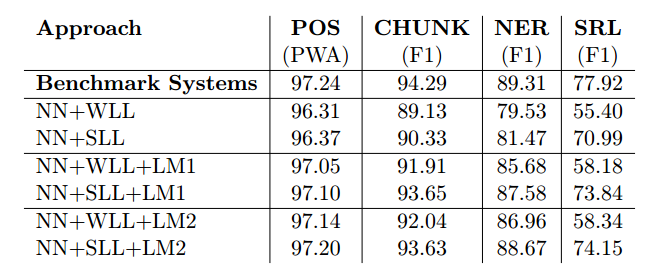
\includegraphics[width=10cm]{cwresults}
  \end{center}
  \begin{enumerate}
  \item Use dense representations instead of sparse
  \item Use windowed area instead of sequence models
  \item Use neural networks to model windowed interactions
  \item Use semi-supervised learning to pretrain representations.
  \end{enumerate}
\end{frame}

\section{word2vec}

\begin{frame}{word2vec}
  \begin{itemize}
  \item Contributions:
    \begin{itemize}
    \item Scale embedding process to massive sizes
    \item Experiments with several architectures
    \item Empirical evaluations of embeddings
    \item Influential release of software/data.
    \end{itemize}
    \pause

  \item Differences with C\&W
    \begin{itemize}
    \item Instead of MLP uses (bi)linear model (linear in paper)
    \item Instead of ranking model, directly predict word (cross-entropy)
    \item Various other extensions.
    \end{itemize}

  \item Two different models
    \begin{enumerate}
    \item Continuous Bag-of-Words (CBOW)
    \item Continuous Skip-gram
    \end{enumerate}



  \end{itemize}
\end{frame}


\begin{frame}{word2vec (Bilinear Model)}
  Back to pure bilinear model, but with much bigger output space
  \[\hat{\boldy} = \softmax((\frac{\sum_{i} \boldx_i^0 \boldW^0}{\dwin-1}) \boldW^1)\]
  \begin{itemize}
  \item $\boldx^0_i \in \reals^{1 \times d_0}$ input words one-hot vectors .
  \item $\boldW^0 \in \reals^{d_0 \times \din}$; $d_0 = |\mcV|$, word embeddings
  \item $\boldW^1 \in \reals^{\din \times \dout}$; $d_{out} = |\mcV|$ output embeddings
  \end{itemize}
  \air
  Notes:
  \begin{itemize}
  \item Bilinear parameter interaction.
  \item $d_0 >> \din$, e.g.  $50 \leq \din \leq 1000$, $10000 \leq |\mcV| \leq 1M$ or more
  \end{itemize}
\end{frame}

\begin{frame}{word2vec (Mikolov, 2013)}
  \begin{center}
    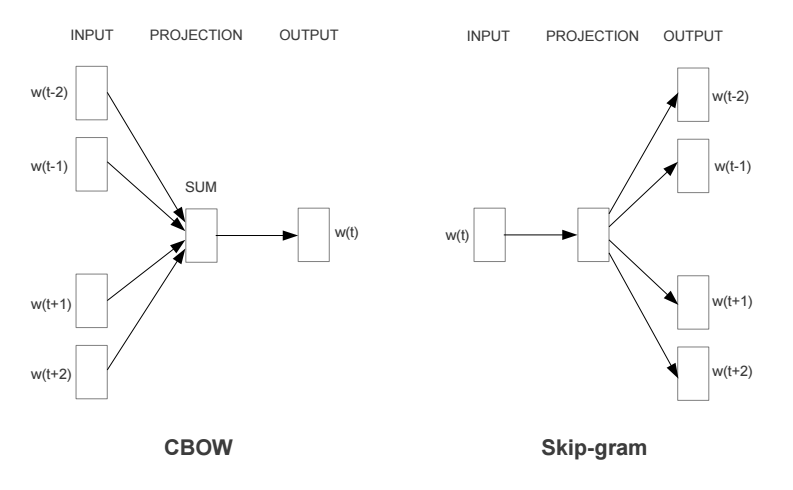
\includegraphics[width=10cm]{word2vec}
  \end{center}
\end{frame}

\begin{frame}{Continuous Bag-of-Words (CBOW) }
  \[\hat{\boldy} = \softmax((\frac{\sum_{i} \boldx_i^0 \boldW^0}{\dwin-1})\boldW^1)\]
  \begin{itemize}

  \item Attempt to predict the middle word
    \begin{center}
      [ \structure{the dog} \alert{walks} \structure{to the} ]
    \end{center}
  \end{itemize}

  Example: CBOW
  \[ \boldx = \frac{v(w_3) +  v(w_4) +   v(w_6) + v(w_7)}{\dwin-1}  \]
  \[ \boldy = \delta(w_5) \]

  % \[\renewcommand\matscale{.6}
  % \matbox{1.5}{4}{\din }{} + \matbox{1.5}{4}{\din }{} + \matbox{1.5}{4}{\din }{\boldx} + \matbox{1.5}{4}{\din }{} + \matbox{1.5}{4}{\din }{}\]

  $\boldW^1$ is no longer partitioned by row (order is lost)
\end{frame}

\begin{frame}{Continous Skip-gram}
  \[\hat{\boldy} = \softmax(\boldx^0 \boldW^0)\boldW^1)\]
  \begin{itemize}
  \item Also a bilinear model
  \item Attempt to predict each context-word from middle

  \begin{center}
    [ \alert{the} \_\_\_ \structure{dog} \_\_\_ \_\_\_  ]
  \end{center}

  \end{itemize}

  Example: Skip-gram
  \[ \boldx = v(w_5)   \]
  \[ \boldy = \delta(w_3)  \]

  Done for each word in window.
\end{frame}


\begin{frame}{Additional aspects}
  \begin{itemize}
  \item The window $\dwin$ is sampled for each SGD step
    \air
  \item SGD is done less for frequent words.
    \air
  \item We have slightly simplified the training objective.
  \end{itemize}
\end{frame}


\begin{frame}{Softmax Issues}
  Use a softmax to force a distribution,

  \[\softmax(\boldz) = \frac{\exp(\boldz)}{\displaystyle \sum_{c\in \mcC } \exp(z_c)}  \]

  \[\log \softmax(\boldz) = \boldz - \log \sum_{c\in \mcC} \exp(z_c)  \]

  \begin{itemize}
  \item \textbf{Issue:} class $\mcC$ is huge.
  \item For C\&W, 100,000, for word2vec 1,000,000 types
  \item Note largest dataset is 6 billion words
  \end{itemize}

\end{frame}

\begin{frame}{Two-Layer Softmax}
  First, clustering words into hard classes (for instance Brown clusters)

  \air

  Groups words into classes based on word-context.
  \begin{center}
    \Tree [ $\ldots$ [ .3 dog cat horse $\ldots$ ] $\ldots$ [ .5 car
    truck motorcycle $\ldots$ ] ]
  \end{center}




\end{frame}

\begin{frame}{Two-Layer Softmax}
  Assume that we first generate a class $C$ and then a word,
  \[p(Y |X) \approx P(Y | C, X;\theta) P(C | X; \theta)\]


  Estimate distributions with a shared embedding layer,

  $P(C |X;\theta)$
  \[\hat{\boldy}_1 = \softmax((\boldx^0 \boldW^0)\boldW^1 + \boldb)\]


  $P(Y | C=class, X;\theta)$
  \[\hat{\boldy}_2 = \softmax((\boldx^0 \boldW^0)\boldW^{class} + \boldb))\]
\end{frame}

\begin{frame}{Softmax as Tree}
  \begin{center}
    \Tree [ $\ldots$ [ .\alert{3} \alert{dog} cat horse $\ldots$ ] $\ldots$ [ .5 car
    truck motorcycle $\ldots$ ] ]
  \end{center}
  \[\hat{\boldy}^{(1)} = \softmax((\boldx^0 \boldW^0)\boldW^1 + \boldb)\]


  \[\hat{\boldy}^{(2)} = \softmax((\boldx^0 \boldW^0)\boldW^{class} + \boldb))\]
  \begin{eqnarray*}
    L_{2SM}(\boldy^{(1)}, \boldy^{(2)}, \hat{\boldy}^{(1)}, \hat{\boldy}^{(2)}) &=& -\log p(\boldy | \boldx, class(\boldy)) -\log p(class(\boldy) | \boldx)  \\
    &=& - \log \hat{y}^{(1)}_{c^{{1}}} - \log \hat{y}^{(2)}_{c^{{2}}} \\
  \end{eqnarray*}
\end{frame}



\begin{frame}{Speed}
  \begin{center}
    \Tree [ $\ldots$ [ .\structure{3} \structure{dog cat horse $\ldots$} ] $\ldots$ [ .5 car
    truck motorcycle $\ldots$ ] ]
  \end{center}
  \begin{itemize}
  \item Computing loss only requires walking path.
    \air
  \item Two-layer a balanced tree.
    \air
  \item Computing loss requires $O(\sqrt{ |\mcV|})$

    \air
  \item (Note: computing full distribution requires $O(|\mcV|)$)

  \end{itemize}

\end{frame}


\begin{frame}{Hierarchical Softmax(HSM) }
  \begin{itemize}
    \item Build multiple layer tree

      \begin{eqnarray*}
        L_{HSM}(\boldy^{(1)}, \ldots,  \boldy^{(C)}, \hat{\boldy}^{(1)}, \ldots,  \hat{\boldy}^{(C)})
                                                                                    &=& - \sum_{i} \log \hat{y}^{(i)}_{c^{{i}}}  \\
      \end{eqnarray*}


  \item Balanced tree only requires $O(\log_2 |\mcV|)$

  \air
  \item Experiments on website (Mnih and Hinton, 2008)
  \end{itemize}
\end{frame}

\begin{frame}{HSM with Huffman Encoding}
  \begin{center}
    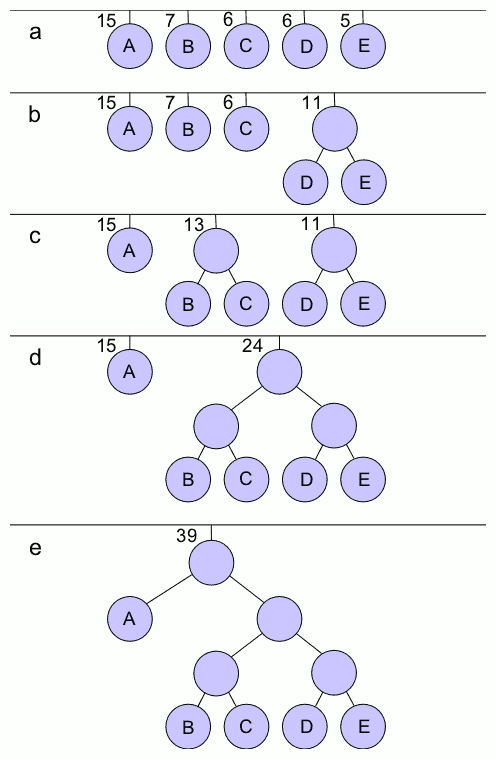
\includegraphics[width=3cm]{HuffmanCodeAlg}
  \end{center}
  \begin{itemize}

  \item Requires $O(\log_2 perp(unigram))$
  \item Reduces time to only 1 day for 1.6 million tokens
  \end{itemize}

\end{frame}

\begin{frame}
  \vspace{-5cm}

  \hspace*{-2cm}
  \includegraphics[width=1.5\textwidth]{../notebooks/graph}
\end{frame}


\section{Evaluating Embeddings}

\begin{frame}{How good are embeddings?}
  \begin{itemize}
  \item Qualitative Analysis/Visualization
    \air
  \item Analogy task
    \air
  \item
    \air
  \item Extrinsic Metrics

  \end{itemize}
\end{frame}

\begin{frame}{Metrics}

  Dot-product

  \[\boldx_{cat} \boldx_{dog}^{\top}\]

  Cosine Similarity

  \[\frac{\boldx_{cat} \boldx_{dog}^{\top}}{||\boldx_{cat} ||\ || \boldx_{dog}||  }\]

\end{frame}

\begin{frame}{k-nearest neighbors (cosine sim)}
  \begin{center}
    dog
    \begin{tabular}{ll}
      cat &  0.921800527377\\
      dogs & 0.851315870426 \\
      horse & 0.790758298322 \\
      puppy & 0.775492121034 \\
      pet & 0.772470734611 \\
      rabbit& 0.772081457265 \\
      pig& 0.749006160038 \\
      snake & 0.73991884888 \\
    \end{tabular}
  \end{center}

  \begin{itemize}
  \item Intuition: trained to match words that act the same.
  \end{itemize}
\end{frame}

\begin{frame}{Empirical Measures: Analogy task }
  Analogy questions:

  \begin{center}
    {\large \texttt{A:B::C:\_\_} }
  \end{center}


  \begin{itemize}
  \item 5 types of semantic questions, 9 types of syntactic
  \end{itemize}
\end{frame}

\begin{frame}{Embedding Tasks}
  \begin{center}
    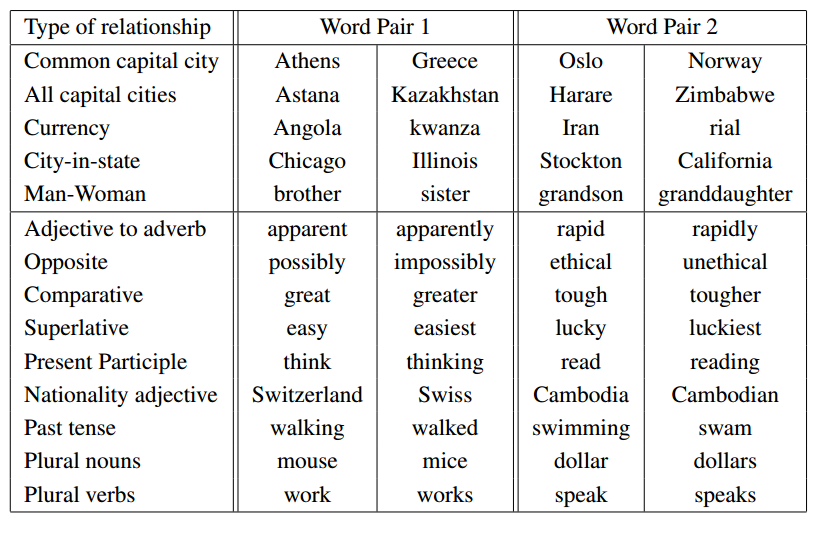
\includegraphics[width=10cm]{analogy}
  \end{center}
\end{frame}


\begin{frame}{Analogy Prediction}

  \begin{center}
    {\large \texttt{A:B::C:\_\_} }
  \end{center}

  \[ \boldx' = \boldx_{B} - \boldx_{A} + \boldx_{C} \]

  Project to the closest word,
  \[ \argmax_{D \in \mcV}\frac{\boldx_{D} \boldx'^{\top}}{||\boldx_{D} || || \boldx'||  } \]

  \begin{itemize}
  \item Code example
  \end{itemize}
\end{frame}

\begin{frame}{Extrinsic Tasks}
  \begin{itemize}
  \item Text classification
    \air

  \item Part-of-speech tagging
    \air


  \item Many, many others over last couple years
  \end{itemize}
\end{frame}

\begin{frame}{Conclusion}
  \begin{itemize}
  \item Word Embeddings
    \air
  \item Scaling issues and tricks

    \air
  \item Next Class: Language Modeling
  \end{itemize}
\end{frame}


\end{document}
